% References:
%   [1] https://tex.stackexchange.com/questions/118069/how-to-draw-an-euler-angle-rotation-sequence-with-tikz

% ---------
% Preamble.
% ---------

% document type
\documentclass{article}

% import custom style
\usepackage{../.preamble/tikz_diagrams_template}

% color theme (black, red, blue, green, orange, purple, gold)
\colortheme{blue}

% ---------
% Document.
% ---------

\begin{document}

    % sets viewing orientation (declination/rotation) of 3D coordinate system
    \tdplotsetmaincoords{90}{0}

    % change rotation matrix to use 3-2-1 sequence
    \tdseteulerxyz

    % -----------------
    % TikZ environment.
    % -----------------

    \begin{tikzpicture}[tdplot_main_coords,scale=1]

        % airplane drawing
        \node[anchor=south west,inner sep=0] (image) at (0,0) {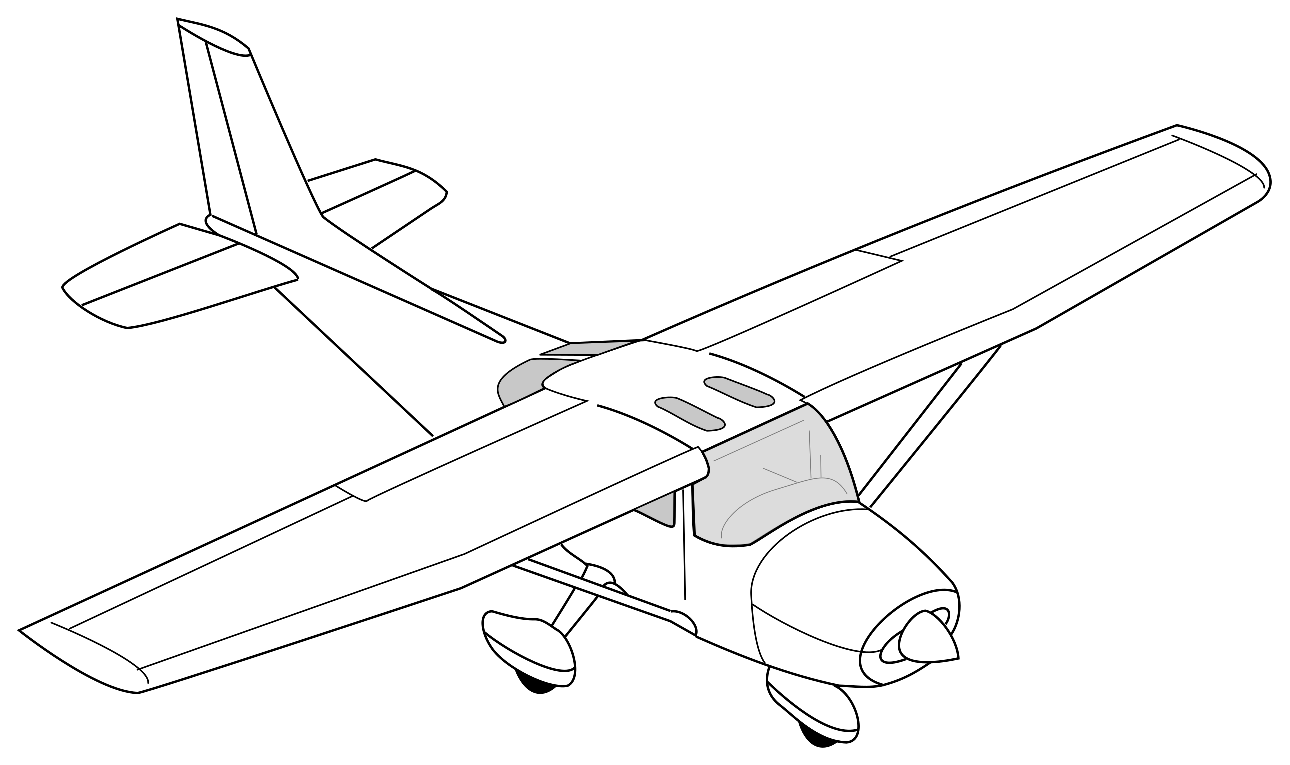
\includegraphics[width=0.6\textwidth]{../.images/airplane.eps}};

        % rotation angles [deg]
        \pgfmathsetmacro{\zRot}{41}
        \pgfmathsetmacro{\yRot}{20}
        \pgfmathsetmacro{\xRot}{-20}
        
        % scope to draw on top of airplane
        \begin{scope}[x={(image.south east)},y={(image.north west)}]
        
            % rotates TikZ's coordinate system to align with body frame
            \tdplotsetrotatedcoords{\zRot}{\yRot}{\xRot}

            % origin
            \pgfmathsetmacro{\Ox}{7.5}
            \pgfmathsetmacro{\Oy}{-0}
            \pgfmathsetmacro{\Oz}{4.84}

            % axes length
            \pgfmathsetmacro{\axlen}{4}
            
            % body axes
            \draw[tdplot_rotated_coords,color_theme,line width=0.5mm](\Ox,\Oy,\Oz)--(\Ox+\axlen,\Oy,\Oz)node[pos=1.08]{$x_{b}$};
            \draw[tdplot_rotated_coords,color_theme,line width=0.5mm](\Ox,\Oy,\Oz)--(\Ox,\Oy+\axlen,\Oz)node[pos=1.1]{$y_{b}$};
            \draw[tdplot_rotated_coords,color_theme,line width=0.5mm](\Ox,\Oy,\Oz)--(\Ox,\Oy,\Oz-\axlen)node[pos=1.08]{$z_{b}$};

            % center of mass
            \node[draw=none,shape=circle,fill,inner sep=1.75pt,color_theme,tdplot_rotated_coords](d1)at(\Ox,\Oy,\Oz){};
            \node[xshift=9,yshift=5,color_theme,tdplot_rotated_coords]at(\Ox,\Oy,\Oz){$\mathrm{cm}$};

        \end{scope}

    \end{tikzpicture}

\end{document}